\chapter{Introduction}

An important technique within the context of text mining is to map words to vectors. Those 
word embeddings can be used as features in statistical models to do further analyses. 
GloVe is a technique to create word embeddings out of a given corpus. A very interesting 
fact is that we want to learn from text without having labels. Hence, we have an unsupervised 
task. \\

Word vectors should be able to represent the human understanding of text in a very 
basic way. That means that word vectors should be able to display the analogy of different 
words as well as general semantic questions. How this is achieved shows image \ref{fig:wv}. 

\begin{figure}[!h]
\centering
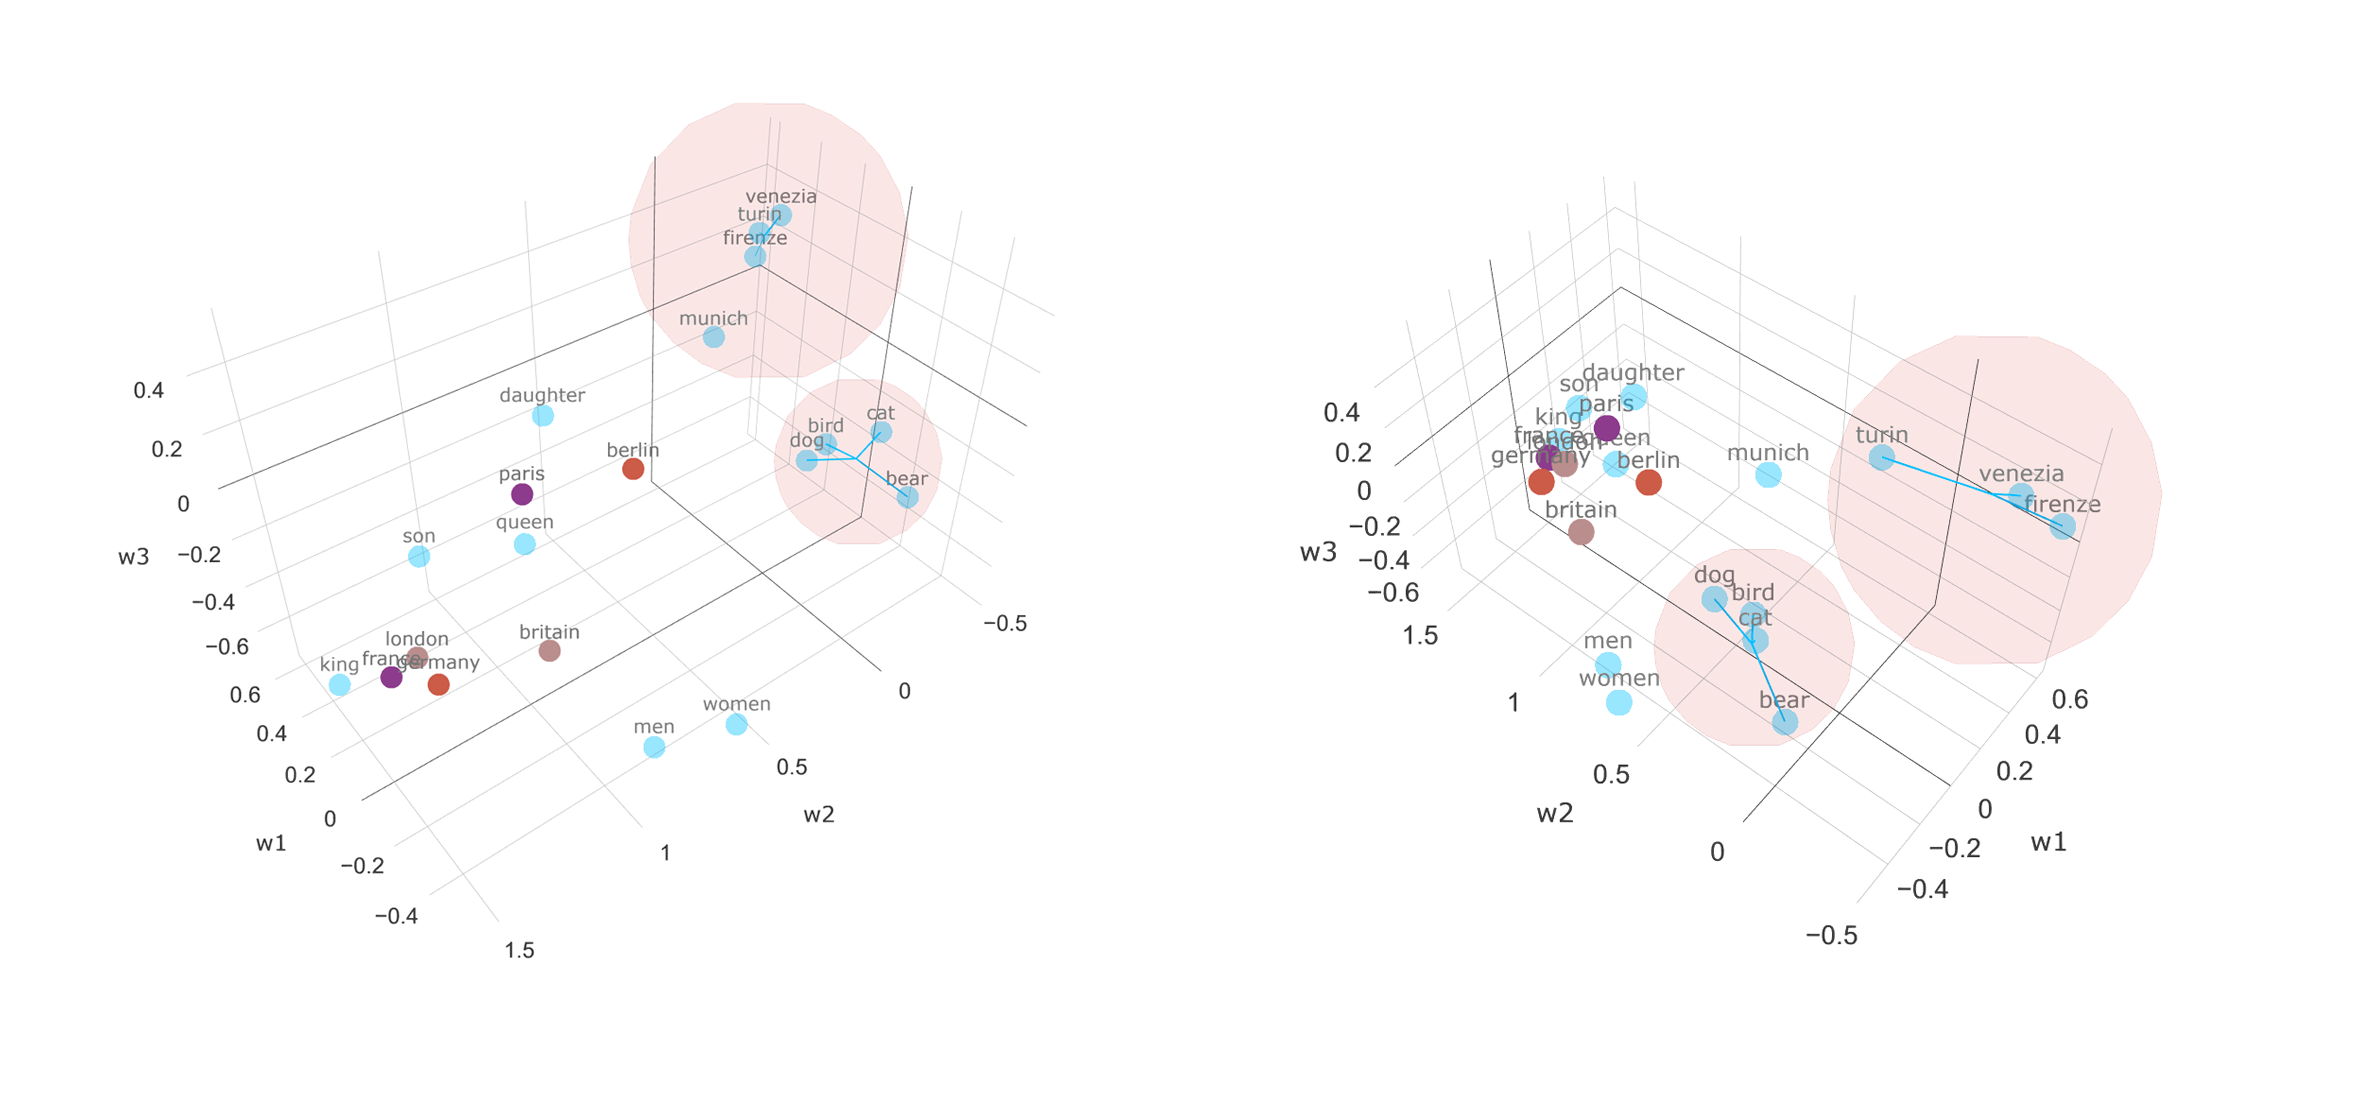
\includegraphics[scale=0.7]{images/wv_glove.png} 
\caption[Word vectors in 3 dimensions trained by GloVe.]{Semantic analogies are stored within 
         the difference of word vectors. For instance, the \enquote{is capital} context is
         represented by the difference between \enquote{france and paris} or 
         \enquote{germany and berlin} which looks very similar. Nevertheless, 
         the \enquote{britian and london} difference looks very different. Hence, a high
         dimension is used for word vectors (e.~g.~300 or 500). Additionally, we want that 
         the word vectors build cluster to related words (e.~g.~italian cities or animals).}
\label{fig:wv}
\end{figure}

In the following we want to discuss some important topics related to GloVe. After 
deriving the model in section \ref{ch:glove} we take a look at how 
to evaluating given word vectors in section \ref{ch:eval} which is quite interesting 
since we handle an unsupervised task. After that we take a short look at the data 
and common sources for text corpora in section \ref{ch:data}. \\

Then we know how to evaluate word vectors and have an idea about the data. With that 
knowledge we may ask how the dimension or different data 
sources influences the quality of the word vectors. This is discussed shortly in section
\ref{ch:real_wv}. After that we give an outlook on how GloVe embeddings can be used for
further text classification techniques followed from a small conclusion in section
\ref{ch:conclusion}.
